\section{Acht varianten en de bijdrage van kenmerken}\label{app:features}
De tabellen en husseltests onderbouwen RQ3. D zijn afstanden, S Shin-richtingen, E eigen categorieën en J wereldgewrichtsmetingen (bijlage A). Alle acht varianten gebruiken dezelfde 60.251 geaccepteerde beelden en dezelfde vijf folds.

\begin{table}[h]\centering\small
\caption{Gepoolde classificatiescores. P is macro-precisie in procenten. J gebruikt wereldpunten; E bevat 70 categoriewaarden voor de 19 eigen controles.}
\begin{tabular}{lrrrrr}\toprule
 & & \multicolumn{2}{c}{SVM} & \multicolumn{2}{c}{LightGBM}\\
Variant & Inputs & P (\%) & Macro-F1 & P (\%) & Macro-F1\\\midrule
\tableinput factorial_summary_rows_nl.tex
\bottomrule\end{tabular}\end{table}

\begin{table}[h]\centering\small
\caption{Herstel en verlies tegenover DS, op dezelfde beelden. Netto is herstel min verlies. Alle vier contexten van elke afzonderlijke toevoeging staan in \texttt{factor\_effects.csv}; de tabel vergelijkt iedere variant met dezelfde basis.}
\begin{tabular}{lrrrrrr}\toprule
 & \multicolumn{3}{c}{SVM} & \multicolumn{3}{c}{LightGBM}\\
Variant & Herstel & Verlies & Netto & Herstel & Verlies & Netto\\\midrule
\tableinput factorial_paired_rows_nl.tex
\bottomrule\end{tabular}\end{table}

\subsection{Controle op de coördinatenbron}
D/S zijn berekend uit beeldhandpunten, E/J uit wereldhandpunten. De onderstaande controle gebruikt voor de gewrichtsmetingen precies dezelfde beeldpunten als Shin, zonder aspectcorrectie. Zij heeft dezelfde bronnen, folds en modelprofielen. De SVM-winst van DSJ met wereldpunten is netto +67, tegenover +4 met deze beeldpunten. De hoekformule alleen verklaart de wereldpuntwinst dus niet.

\begin{table}[h]\centering\small
\caption{Controles met J uit beeldpunten; geen eigen categorieën toegevoegd. Dit zijn aanvullende controles, niet twee extra hoofdvarianten.}
\begin{tabular}{lrrrr}\toprule
 & \multicolumn{2}{c}{SVM} & \multicolumn{2}{c}{LightGBM}\\
Variant & P (\%) & Macro-F1 & P (\%) & Macro-F1\\\midrule
\tableinput factorial_controls_nl.tex
\bottomrule\end{tabular}\end{table}

De tabellen vergelijken E en J afzonderlijk en samen, steeds met en zonder S. De uitkomsten gelden voor de vaste profielen en deze bronnen; een rangorde bewijst geen universeel beste featurebeschrijving.

\clearpage
\subsection{Permutatietests na het trainen}
Per fold zijn vooraf met seed 20261107 honderd toetsbeelden per letter gekozen: 2.600 per fold en 13.000 unieke beelden totaal. Alle modellen gebruiken dezelfde subset. Dit is een aparte, kleinere noemer dan de volledige classificatievergelijking. Per groep worden de waarden met vijf vaste rijpermutaties tussen toetsbeelden verwisseld. Labels blijven gelijk; het foldmodel wordt niet opnieuw getraind.

\begin{figure}[h]\centering
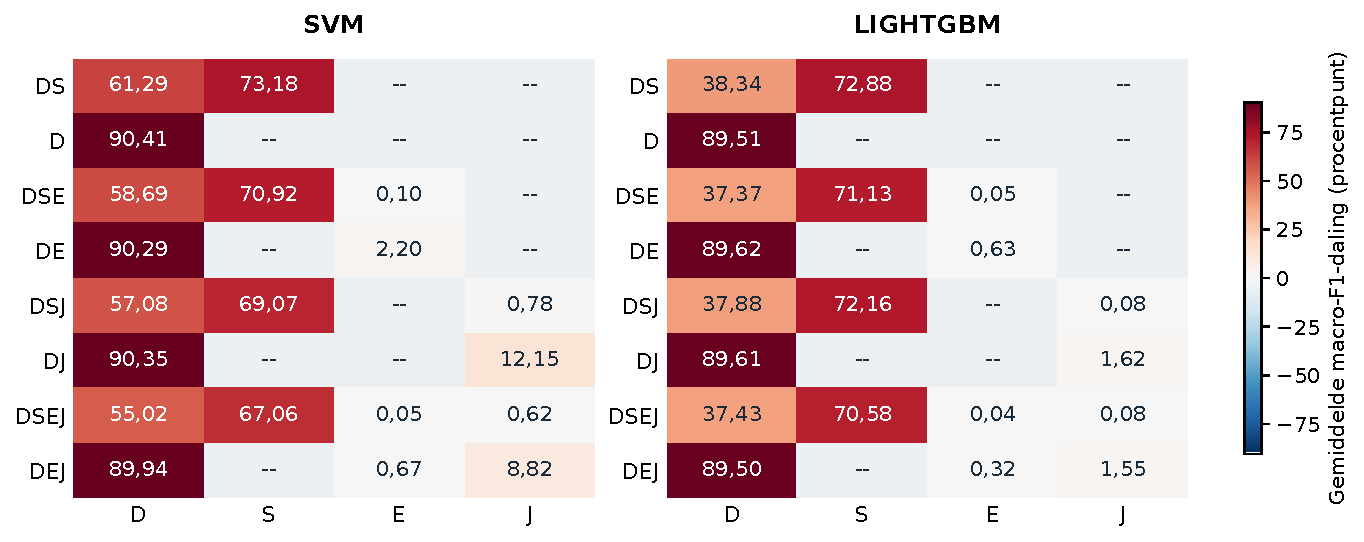
\includegraphics[width=.96\linewidth,height=.31\textheight,keepaspectratio]{figures/factorial_block_importance.pdf}
\caption{Grote featureblokken in iedere variant. Getallen zijn de gemiddelde daling van macro-F1 in procentpunten over vijf folds en vijf husselingen; één punt is 0,01 F1. -- betekent dat het blok ontbreekt. Een grote positieve daling duidt op afhankelijkheid van dat blok onder deze verstoring.}
\end{figure}

\begin{figure}[h]\centering
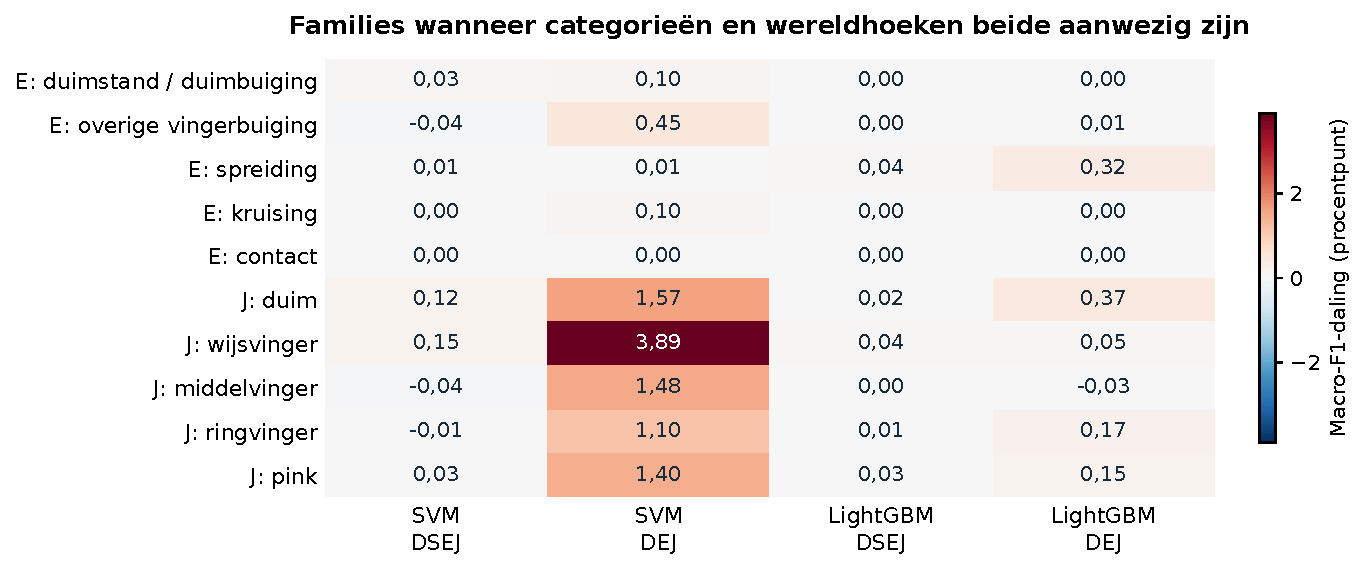
\includegraphics[width=.96\linewidth,height=.32\textheight,keepaspectratio]{figures/factorial_family_importance.pdf}
\caption{Vijf categorische families (E) en vijf gewrichtsfamilies (J) wanneer beide aanwezig zijn. Elke familie wordt gezamenlijk gehusseld. S kan informatie uit de toevoegingen deels vervangen, en omgekeerd. Een negatieve daling wordt behouden: die husseling verbeterde de score gemiddeld.}
\end{figure}

Alle kolommen binnen een groep volgen dezelfde rijpermutatie. Zo blijft een one-hot vector geldig. Fold/herhaling delen dezelfde volgorde over varianten en leermethoden. De SVM-uitvoering hergebruikt equivalente RBF-afstanden; oorspronkelijke voorspellingen en verstoorde gevallen worden tegen de gewone SVC-route gecontroleerd. Seeds en uitvoering staan in \texttt{protocol.json} en \texttt{execution\_backend.json}. De CSV bevat ook precisiedalingen en beschrijvende spreiding; dit is geen onafhankelijk betrouwbaarheidsinterval.

\clearpage
\subsection{De 19 eigen controles afzonderlijk}
De afzonderlijke categorieën worden in DSE en DE onderzocht, dus zonder J. Dat maakt zichtbaar welke eigen beschrijvingen het model gebruikt wanneer niet tegelijk de directe wereldgewrichtsmetingen aanwezig zijn. De familieproef op de vorige pagina laat de volledige combinaties mét J zien.

\begin{figure}[h]\centering
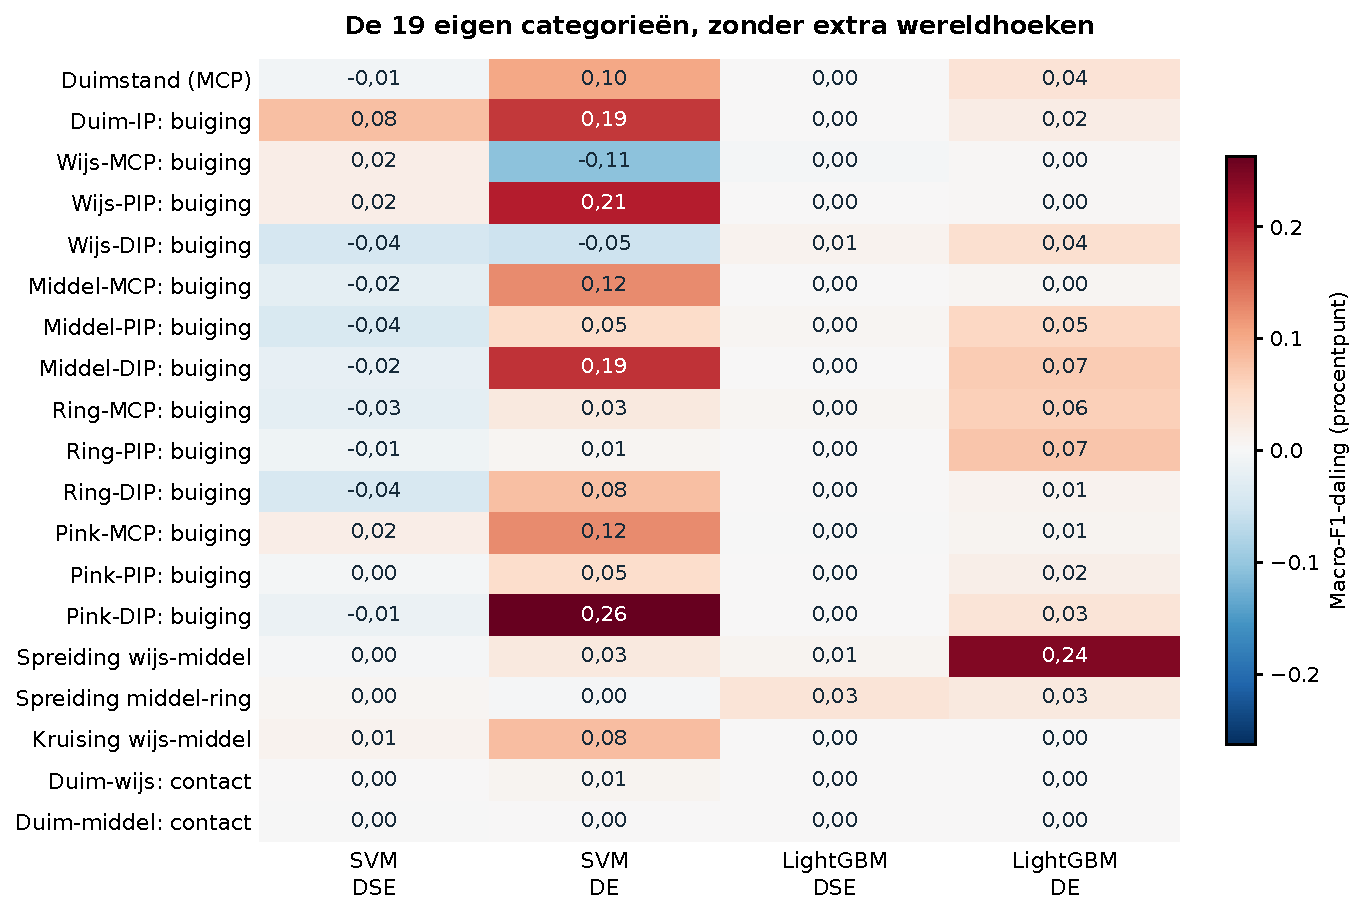
\includegraphics[width=.96\linewidth,height=.58\textheight,keepaspectratio]{figures/factorial_category_importance.pdf}
\caption{Macro-F1-daling per eigen controle, steeds met alle bijbehorende categorie-kolommen samen verwisseld. DSE bevat de Shin-richtingen, DE niet. Gemiddelden zijn berekend op dezelfde 13.000 toetsbeelden en vijf husselingen per fold. De labels verwijzen naar de 19 controles die in bijlage C zijn geïllustreerd.}
\end{figure}

Permutatie meet de afhankelijkheid van een getraind model onder verstoring. Zij meet niet hoeveel extra prestatie een nieuw getraind model door die feature krijgt: daarvoor dienen de acht trainingsvarianten. Samenhangende features kunnen elkaar vervangen, waardoor een nuttig kenmerk weinig afzonderlijke permutatiedaling geeft. Andersom kan een verstoorde groep een ongewone combinatie met andere groepen vormen. Deze resultaten zijn daarom geen causale ranglijst van intrinsiek belangrijke handkenmerken.

Alle fold- en letterscores, verwarringsmatrices, paarsgewijze verschillen, husseluitkomsten en controles staan in \texttt{results/feature\_factorial\_01/}. De opgeslagen modellen worden op toetsgevallen gereplayed en de scores onafhankelijk herberekend. Dit verifieert de uitvoering, niet de handanatomie of generalisatie naar nieuwe personen.
